\chapter{Forschungsergebnisse}

\section{Ergebnisse - Zweiter Implementierungsabschnitt}
\subsection{Rangliste der Evaluationsmetriken}
In den folgenden beiden Tabellen \ref{tab:ZIa-EI-EV-20} und \ref{tab:ZIa-EI-EV-160} sind die Ergebnisse der Evaluationsmetriken für den zweiten Implementierungsabschnitt enthalten, welche nach Rang bzw. aufsteigend nach bester Algorithmus-Kombination geordnet sind. Der Rang ergibt sich dabei aus dem Mittelwert der normalisierten Werte der Metriken (Davies-Bouldin Index invertiert normalisiert). Die optimalen Werte für die verschiedenen Verfahren sind wie folgt:
\begin{itemize}
    \item Silhouette Score: 0,5 oder höher
    \item Caliński-Harabasz Index: höchster Wert aus allen Tests
    \item Davies-Bouldin Index: niedrigster Wert aus allen Tests (gut zwischen 0,3 und 0,7)
\end{itemize}
Tabelle \ref{tab:ZIa-EI-EV-20} legt nahe, dass UMAP das geeignetste Dimensionsreduktionsverfahren ist, unabhängig vom Clustering-Algorithmus, wobei t-SNE und PCA mittelwertige Ergebnisse mit k-Means und schlechtere Ergebnisse mit HDBSCAN liefern.
Tabelle \ref{tab:ZIa-EI-EV-160} zeigt, dass sich die Eignung nicht großartig ändert. So sind sowohl für kleine, als auch große Dateimengen beide Clustering-Algorithmen zusammen mit UMAP geeignet.

\setlength{\tabcolsep}{5.5pt}
\begin{table}[h]
\centering
\begin{tabular}{lcccc}
\hline
\textbf{Kombination} & \textbf{Silhouette} & \textbf{Calinski-Harabasz} & \textbf{Davies-Bouldin} & \textbf{Rang} \\
\hline
umap\_kmeans    & 0.763 & 3593.558 & 0.317 & 1 \\
umap\_hdbscan   & 0.728 & 3248.739 & 0.425 & 2 \\
tsne\_kmeans    & 0.640 & 173.360  & 0.273 & 3 \\
pca\_kmeans     & 0.609 & 168.268  & 0.444 & 4 \\
pca\_hdbscan    & 0.573 & 85.872   & 0.777 & 5 \\
tsne\_hdbscan   & 0.600 & 2.318    & 5.856 & 6 \\
\hline
\end{tabular}
\caption{Zweiter Implementierungsabschnitt - Evaluationsergebnisse mit 40 Dateien.}
\label{tab:ZIa-EI-EV-20}
\end{table}

\setlength{\tabcolsep}{5.5pt}
\begin{table}[h]
\centering
\begin{tabular}{lcccc}
\hline
\textbf{Kombination} & \textbf{Silhouette} & \textbf{Calinski-Harabasz} & \textbf{Davies-Bouldin} & \textbf{Rang} \\
\hline
umap\_kmeans    & 0.595 & 6554.361 & 0.390 & 1 \\
umap\_hdbscan   & 0.671 & 1398.606 & 0.608 & 2 \\
tsne\_kmeans    & 0.579 & 490.225  & 0.609 & 3 \\
pca\_kmeans     & 0.716 & 36.378   & 0.863 & 4 \\
pca\_hdbscan    & 0.408 & 201.754  & 0.780 & 5 \\
tsne\_hdbscan   & 0.421 & 267.712  & 0.814 & 6 \\
\hline
\end{tabular}
\caption{Zweiter Implementierungsabschnitt - Evaluationsergebnisse mit 320 Dateien.}
\label{tab:ZIa-EI-EV-160}
\end{table}


\subsection{Clustern unterschiedlicher Dateien in einem Diagramm}
\label{abs:C-u-D-i-e-D}
Folgende Abbildungen zeigen Clusterungen mit steigender Anzahl Dateien, die sich auf den zweiten Implementierungsabschnitt beziehen. Dabei trat das Problem auf, dass bei größeren Dateimengen die Wahrscheinlichkeit für gemischte Cluster, also mit unterschiedlichen Dateien in einem Cluster anstieg. In den Abbildungen \ref{abb:ZIa-C-160-gC} und \ref{abb:ZIa-C-160-gC-z} ist die Clusterung von 160 Point.java- (orangene Punkte) und 160 Circle.java-Dateien (blaue Punkte) und das beschriebene Problem zu sehen. Die genutzte Algorithmen-Kombination war UMAP mit HDBSCAN. Andere Kombinationen wie PCA mit k-Means ergaben deutlich andere Ergebnisse, jedoch stieg hier die Anzahl der gemischten Cluster ebenso an.

\begin{figure} %[hbtp]
	\centering
	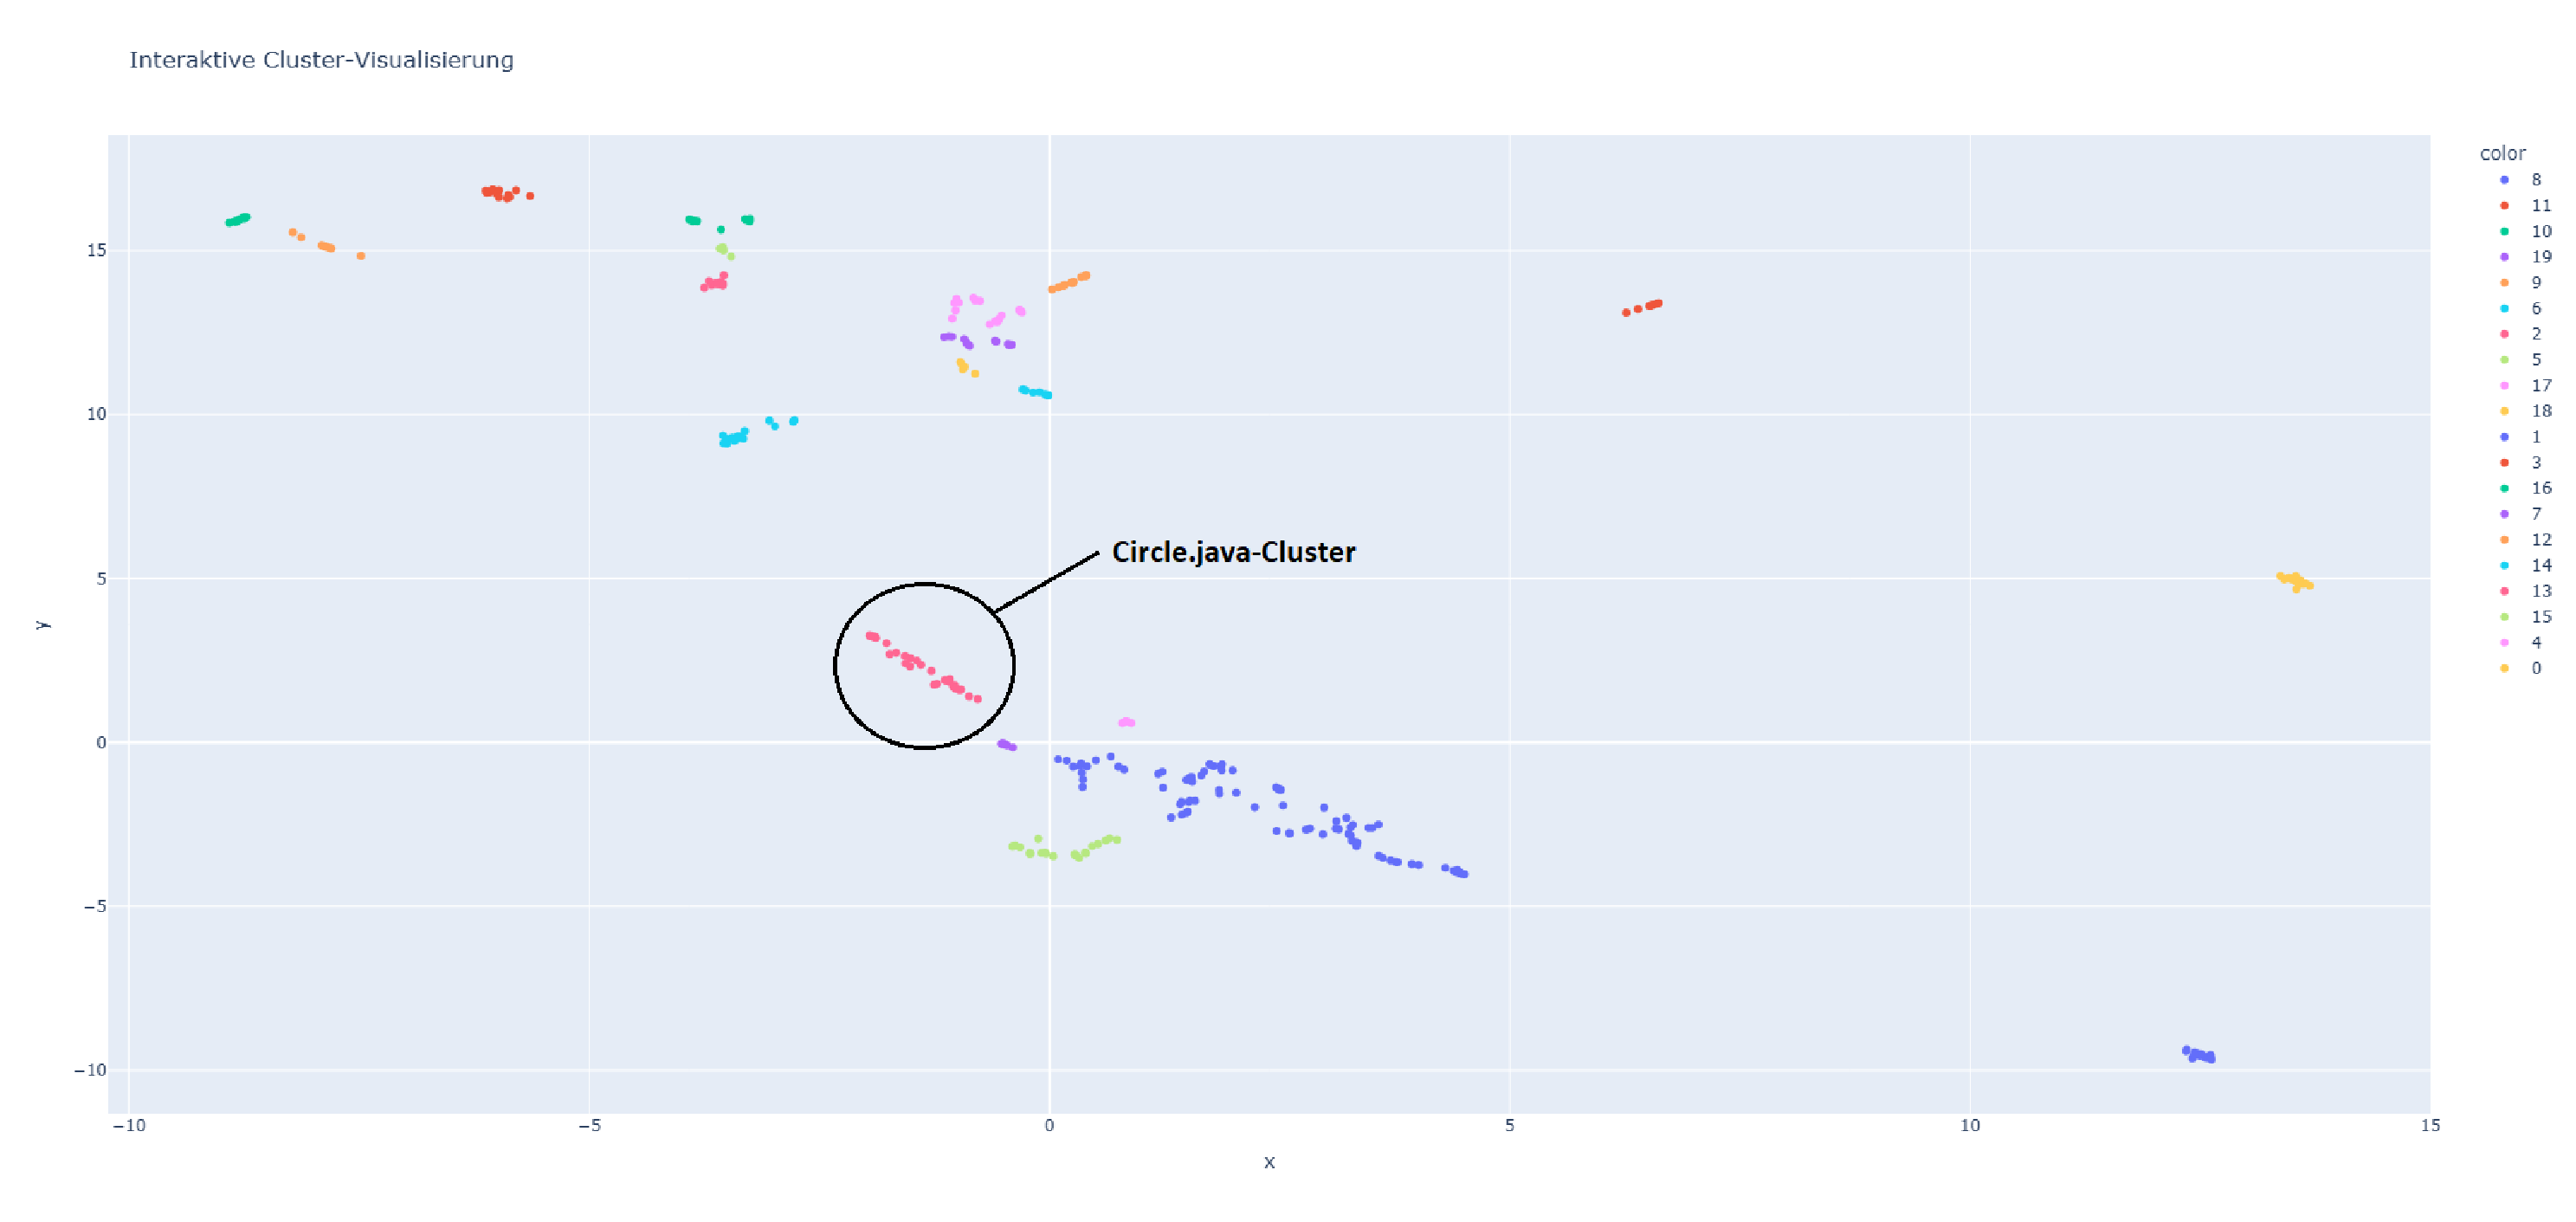
\includegraphics[width=1.0\textwidth]{images/Clusterung - 160 - gemischte Cluster.pdf}
	\caption{Zweiter Implementierungsabschnitt - Clustering-Diagramm einer Clusterung von 320 Java-Dateien. Der eingekreiste Cluster ist ein Circle.java-Cluster.}
	\label{abb:ZIa-C-160-gC}
\end{figure}

\begin{figure} %[hbtp]
	\centering
	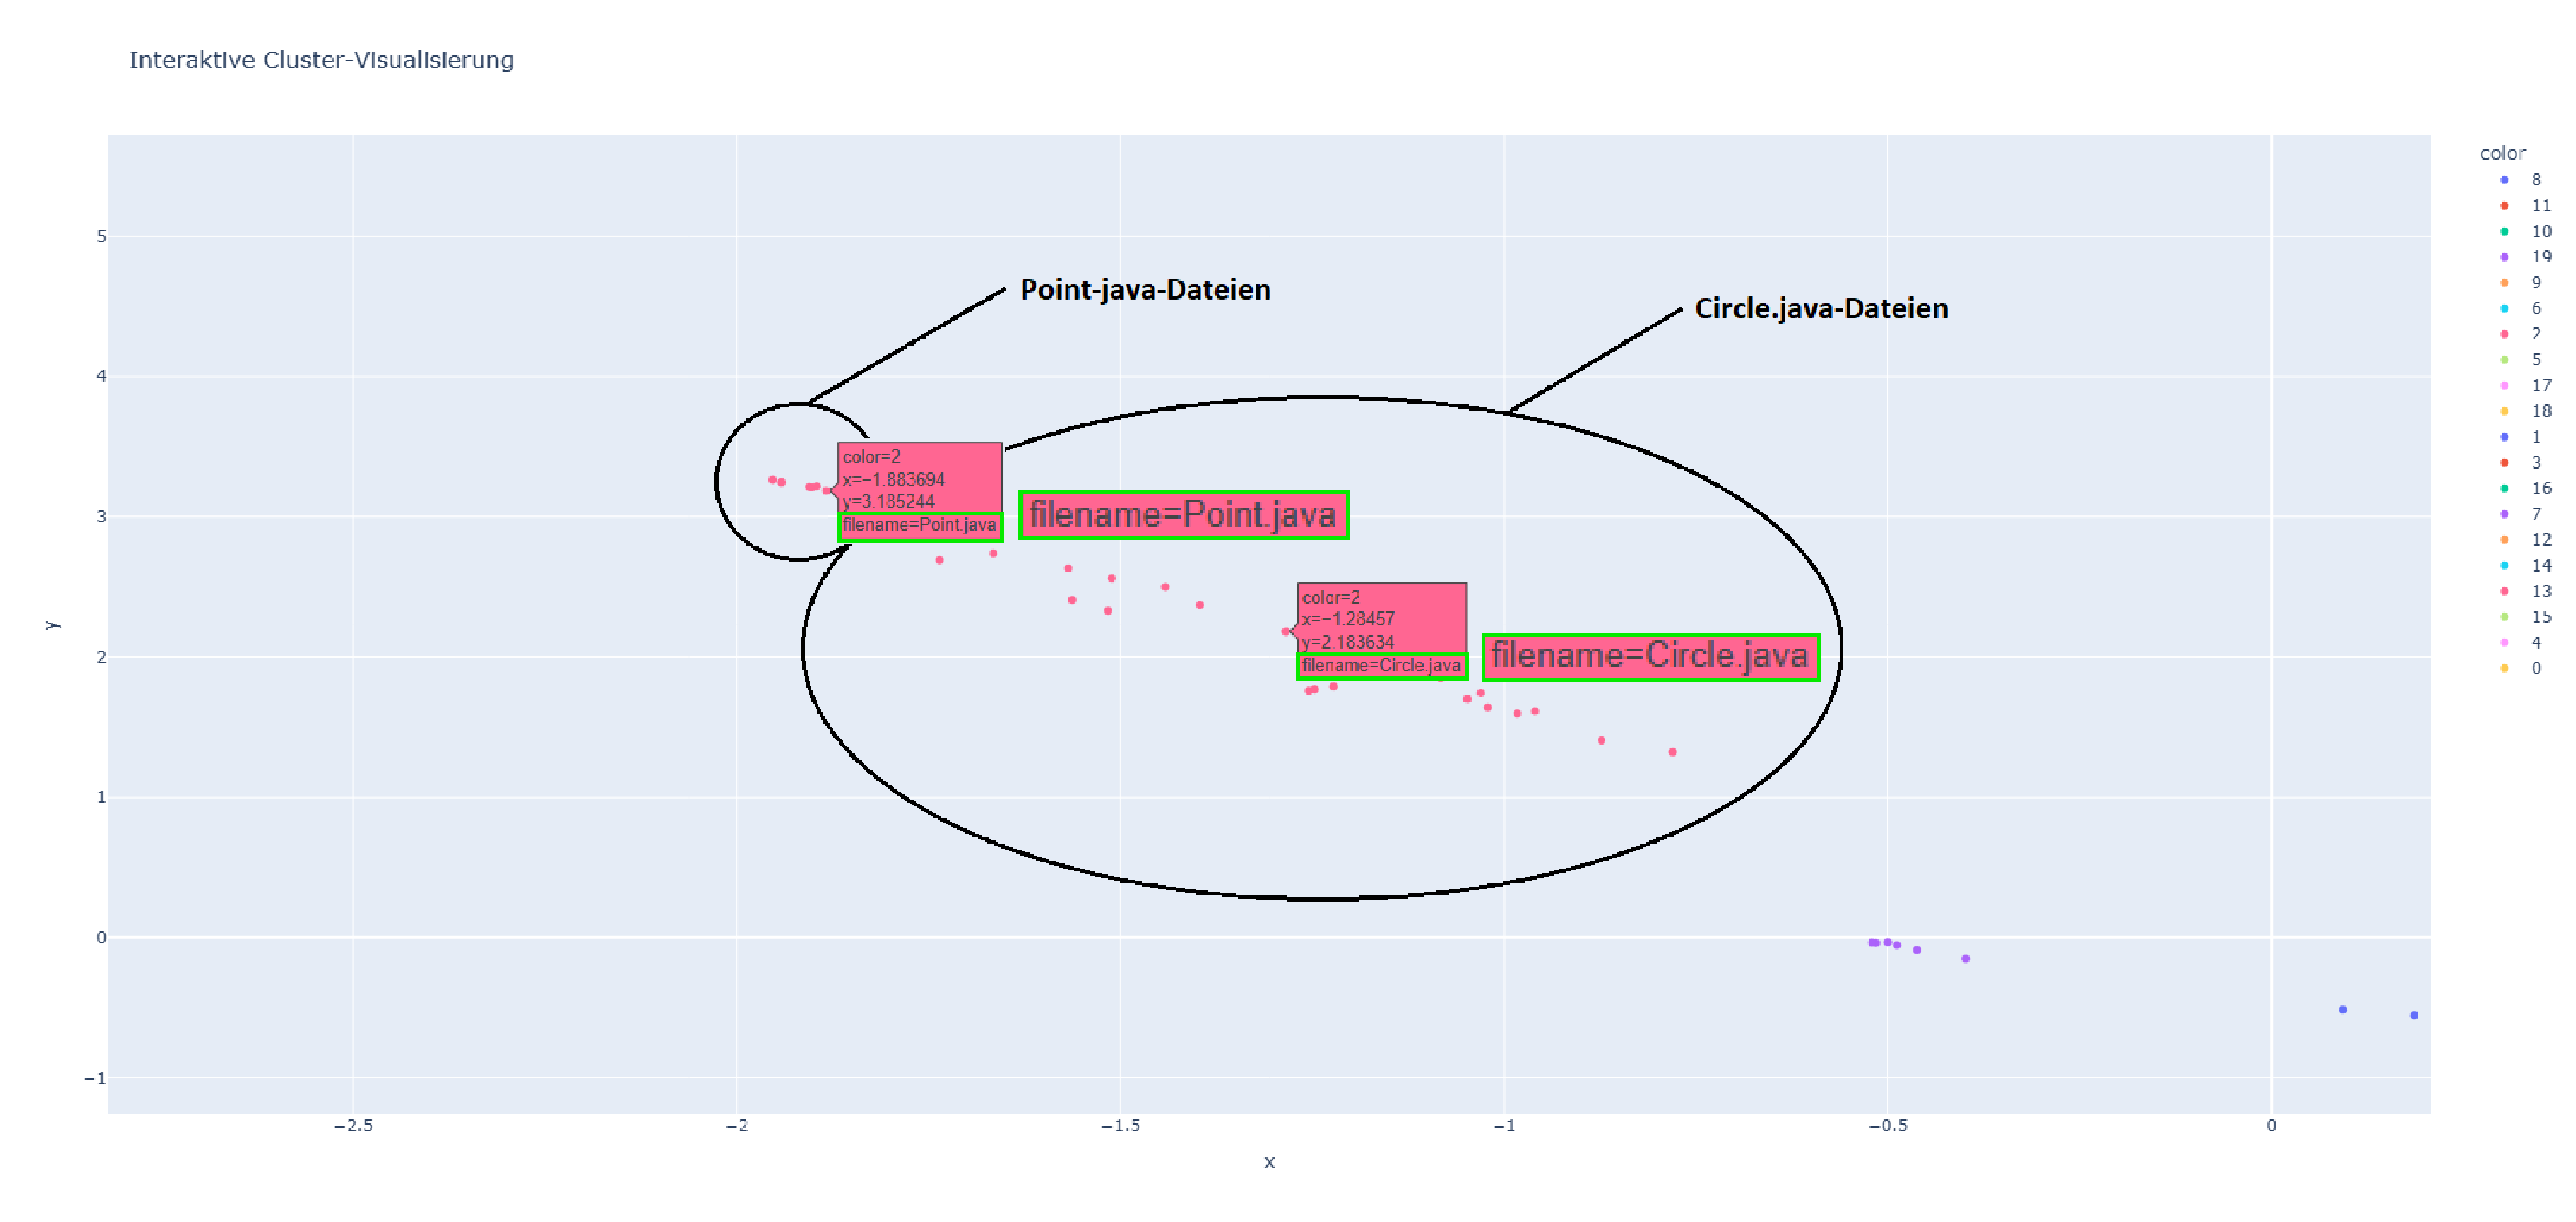
\includegraphics[width=1.0\textwidth]{images/Clusterung - 160 - gemischte Cluster - zoom.pdf}
	\caption{Zweiter Implementierungsabschnitt - Vergrößerter Circle.java-Cluster aus Abbildung \ref{abb:ZIa-C-160-gC}}
	\label{abb:ZIa-C-160-gC-z}
\end{figure}

\section{Ergebnisse - Finale Implementierung}
Anhand der finalen Implementierung kann nun ein realistisches Szenario getestet werden. Die Abbildungen \ref{abb:Miniprojekt-1-S.1} und \ref{abb:Miniprojekt-1-S.2} beschreibt eine beispielhafte Aufgabenstellung:

\begin{figure} %[hbtp]
	\centering
	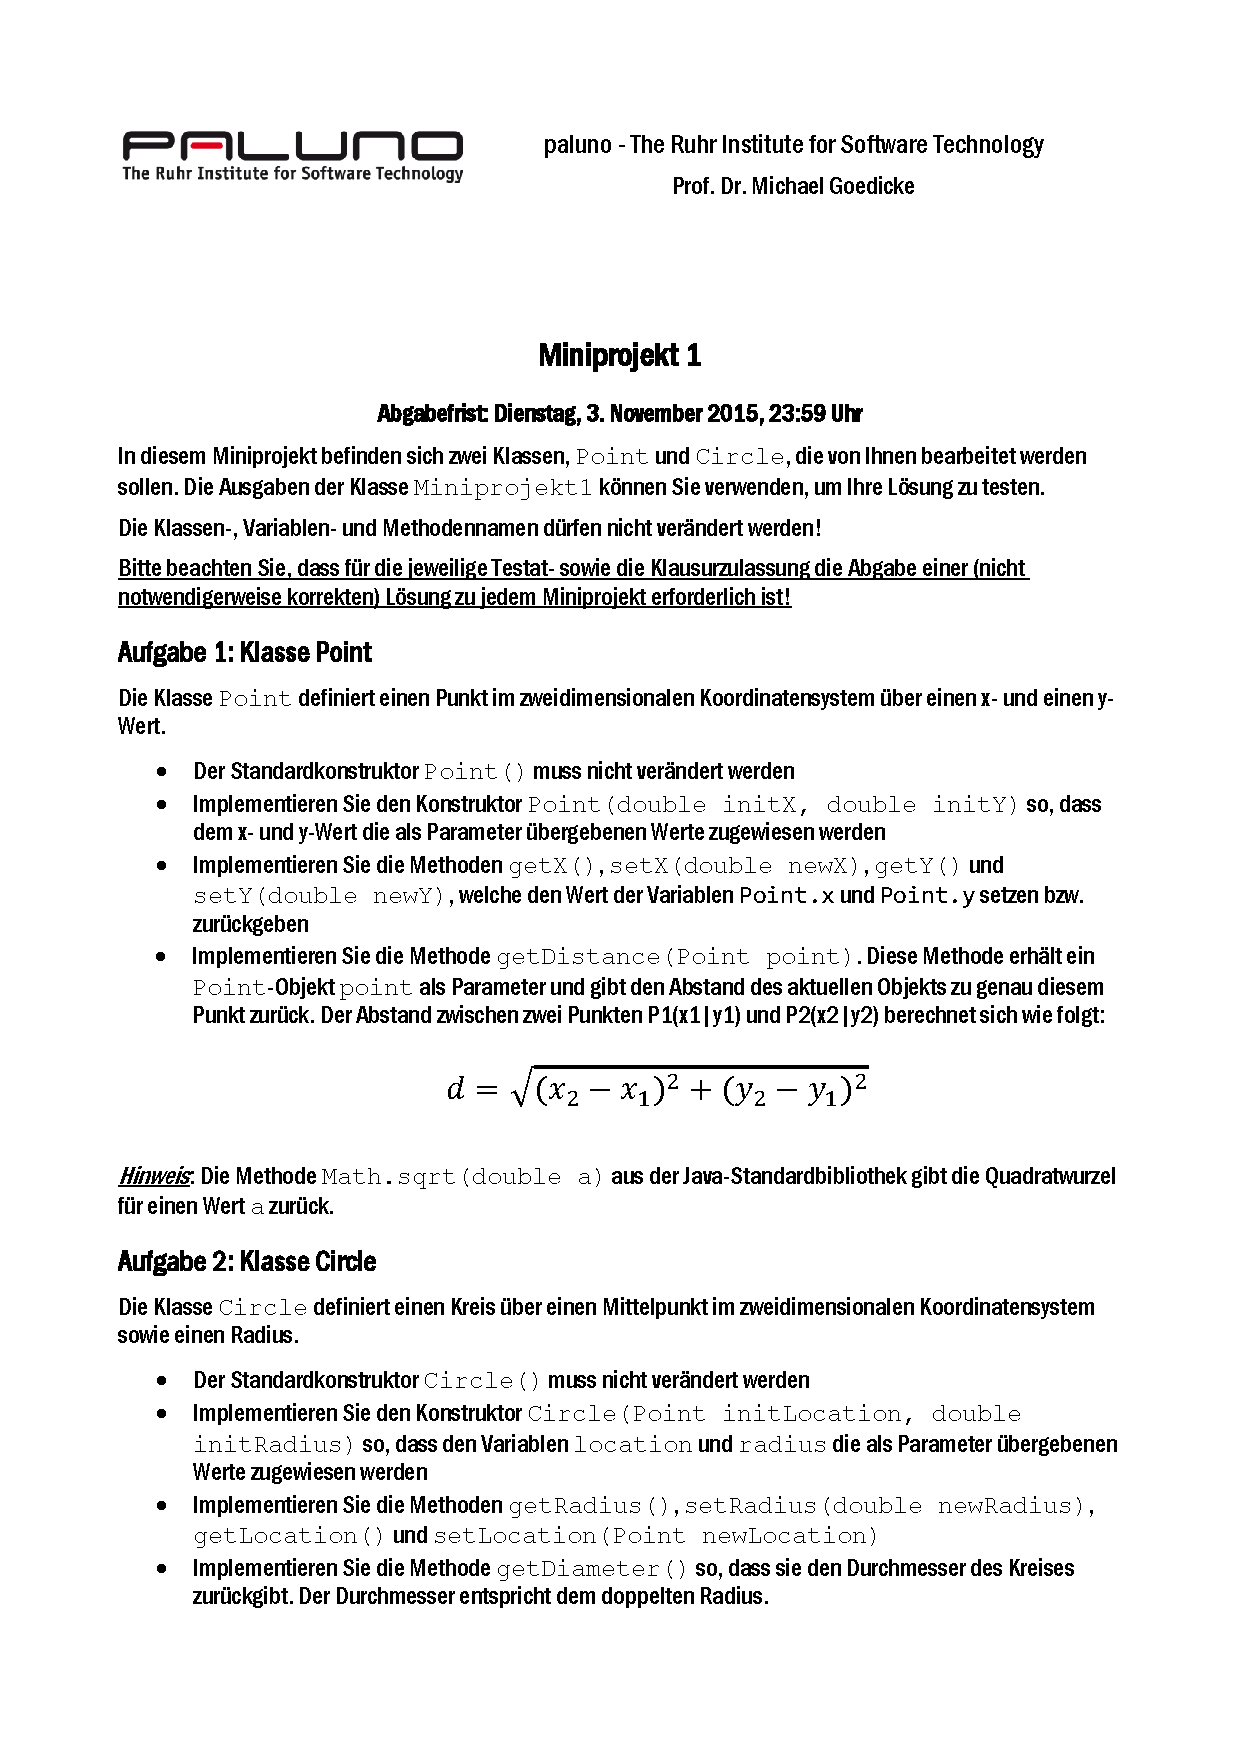
\includegraphics[width=1.0\textwidth]{images/Miniprojekt-1-S.1.pdf}
	\caption{Programmieraufagbe aus dem Jahr 2015 des paluno - The Ruhr Institute for Software Technology von Prof. Dr. Michael Goedicke, erste Seite}
	\label{abb:Miniprojekt-1-S.1}
\end{figure}

\begin{figure} %[hbtp]
	\centering
	
\includegraphics[width=1.0\textwidth]{images/Miniprojekt-1-S.2.pdf}
	\caption{Programmieraufagbe aus dem Jahr 2015 des paluno - The Ruhr Institute for Software Technology von Prof. Dr. Michael Goedicke, zweite Seite}
	\label{abb:Miniprojekt-1-S.2}
\end{figure}

Die zu bearbeitenden Java-Dateien waren Miniprojekt1, Point und Circle. Miniprojekt1-Dateien wurden ignoriert, da sie nicht bearbeitet werden sollten. Gefordert waren die Implementierung verschiedener Methoden der Point und Circle Klassen. Zunächst wurden die Einreichungen anhand der Experimentierungspipeline auf die beste Algorithmen-Kombination anhand Punktzahlenintervalle getestet. Sie wurden an das Notensystem angelehnt definiert (Note 1.0 bis 1.3 $\overset{\wedge}{=}$ Punktzahl $\geq$ 90, Note 1.7 bis 2.3 $\overset{\wedge}{=}$ Punktzahl $\geq$ 75, etc.), wobei perfekte Erebnisse (mit 100 Punkten bewertet) extra geclustert werden. Wenn die Dateimengen oder die Punktzahlenintervalle klein gewählt sind, treten dabei vermehrt Probleme der Algorithmen auf, die mit geringen Datenmengen nicht funktionieren. Deshalb wurde eine Menge von rund 1000 studentischen Einreichungen/Lösungen zum Testen verwendet (entspricht etwa 2000 einzelnen bzw. 1000 konkatenierten Dateien). Tabelle \ref{tab:FI-EI-EV-160-oPI} zeigt die Ergebnisse der Evaluationsmetriken ohne und Tabelle \ref{tab:FI-EI-EV-160-mPI} mit Punktzahlenintervalle. Trotz der Verfälschung in der zweiten Tabelle durch die Punktzahlenintervalle, stellte sich die Kombination UMAP mit k-Means als am besten heraus.

\setlength{\tabcolsep}{5.5pt}
\begin{table}[h]
\centering
\begin{tabular}{lcccc}
\hline
\textbf{Kombination} & \textbf{Silhouette} & \textbf{Calinski-Harabasz} & \textbf{Davies-Bouldin} & \textbf{Rang} \\
umap\_kmeans    & 0.479 & 2417.266 & 0.591 & 1 \\
pca\_kmeans     & 0.530 & 1872.106 & 0.495 & 2 \\
pca\_hdbscan    & 0.702 & 239.336  & 0.343 & 3 \\
tsne\_kmeans    & 0.373 & 1224.132 & 0.924 & 4 \\
umap\_hdbscan   & 0.110 & 845.411  & 0.473 & 5 \\
tsne\_hdbscan   & 0.530 & 40.382   & 1.750 & 6 \\
\hline
\end{tabular}
\caption{Finale Implementierung - Evaluationsergebnisse mit rund 1000 Dateien (ohne Punktzahlenintervalle).}
\label{tab:FI-EI-EV-160-oPI}
\end{table}

\setlength{\tabcolsep}{5.5pt}
\begin{table}[h]
\centering
\begin{tabular}{lcccc}
\hline
\textbf{Kombination} & \textbf{Silhouette} & \textbf{Calinski-Harabasz} & \textbf{Davies-Bouldin} & \textbf{Rang} \\
umap\_hdbscan   & -0.124 & 100.007 & 4.872 & 1 \\
umap\_kmeans    & -0.017 & 25.222  & 6.107 & 2 \\
pca\_kmeans     & -0.006 & 14.737  & 6.880 & 3 \\
pca\_hdbscan    &  0.067 & 17.322  & 9.449 & 4 \\
tsne\_kmeans    & -0.033 & 11.893  & 9.075 & 5 \\
tsne\_hdbscan   & -0.494 & 2.994   & 20.513 & 6 \\
\hline
\end{tabular}
\caption{Finale Implementierung - Evaluationsergebnisse mit rund 1000 Dateien (mit Punktzahlenintervalle).}
\label{tab:FI-EI-EV-160-mPI}
\end{table}

Als nächstes wurde die Pipeline verwendet, um die Clusterungen zu visualisieren. Abbildung \ref{abb:C-1000} zeigt das entstandene Diagramm, wobei die unterschiedlichen Farben und Überlappung der Cluster durch die Punktzahlenintervalle zustande kamen und damit visuell weniger wertvoll sind. Aus diesem Grund wurde auf die erstellte CSV-Datei aus dem cluster\_report zurückgegriffen. Nun galt es zu überprüfen ob für die Cluster jeweils ein identisches Feedback ausreicht. Dafür wurden aus jedem Cluster zwei Kandidaten ausgesucht und nach Fehlerarten gesucht, welche das jeweilige Feedback bestimmen würden. Die Tabellen \ref{tab:A-d-CD}, \ref{tab:A-d-PD} und \ref{tab:Abk} zeigen die Ergebnisse. Die ersten beiden Tabellen stehen dabei für die Auswertung der Circle- und Point-Dateien und die letzte für die verwendeten Abkürzungen. Sie sind sortiert nach Punktzahlenintervalle (Sc.-B.), Cluster, Aufgabenart (C1-C10, P1-P6), Einreichungen (aus Platzgründen zu Punktzahl und "P" abgekürzt, z. B. "53 P") und ob die Antworten gleich oder ungleich waren. Die Ergebnisse zeigen, dass die Zahl der gleichen Antworten nach steigenden Punktzahlenintervallen entsprechend mitwächst. Identisches Feedback ist erst bei einer 100-prozentigen Übereinstimmung der Antworten sinnvoll. Hier wäre es also nur im Bereich 60-74 und 90-99 angebracht identisches Feedback zu generieren. Um mehr gewährleisten zu können, würde womöglich eine weitere Spezialisierung der Punktzahlenintervalle als Idee nahe erscheinen, jedoch wurden bei einer identischen Punktzahl (53 und 53 in Sc.-B. 50-59) nur ungleiche Antworten gegeben. Es ist also eine Verallgemeinerung der Antwortarten oder des Feedbacks notwendig. Weiterhin könnten Tests mit verschiedenen Algorithmen-Kombinationen für präzisere Ergebnisse sorgen.

\begin{figure} %[hbtp]
	\centering
	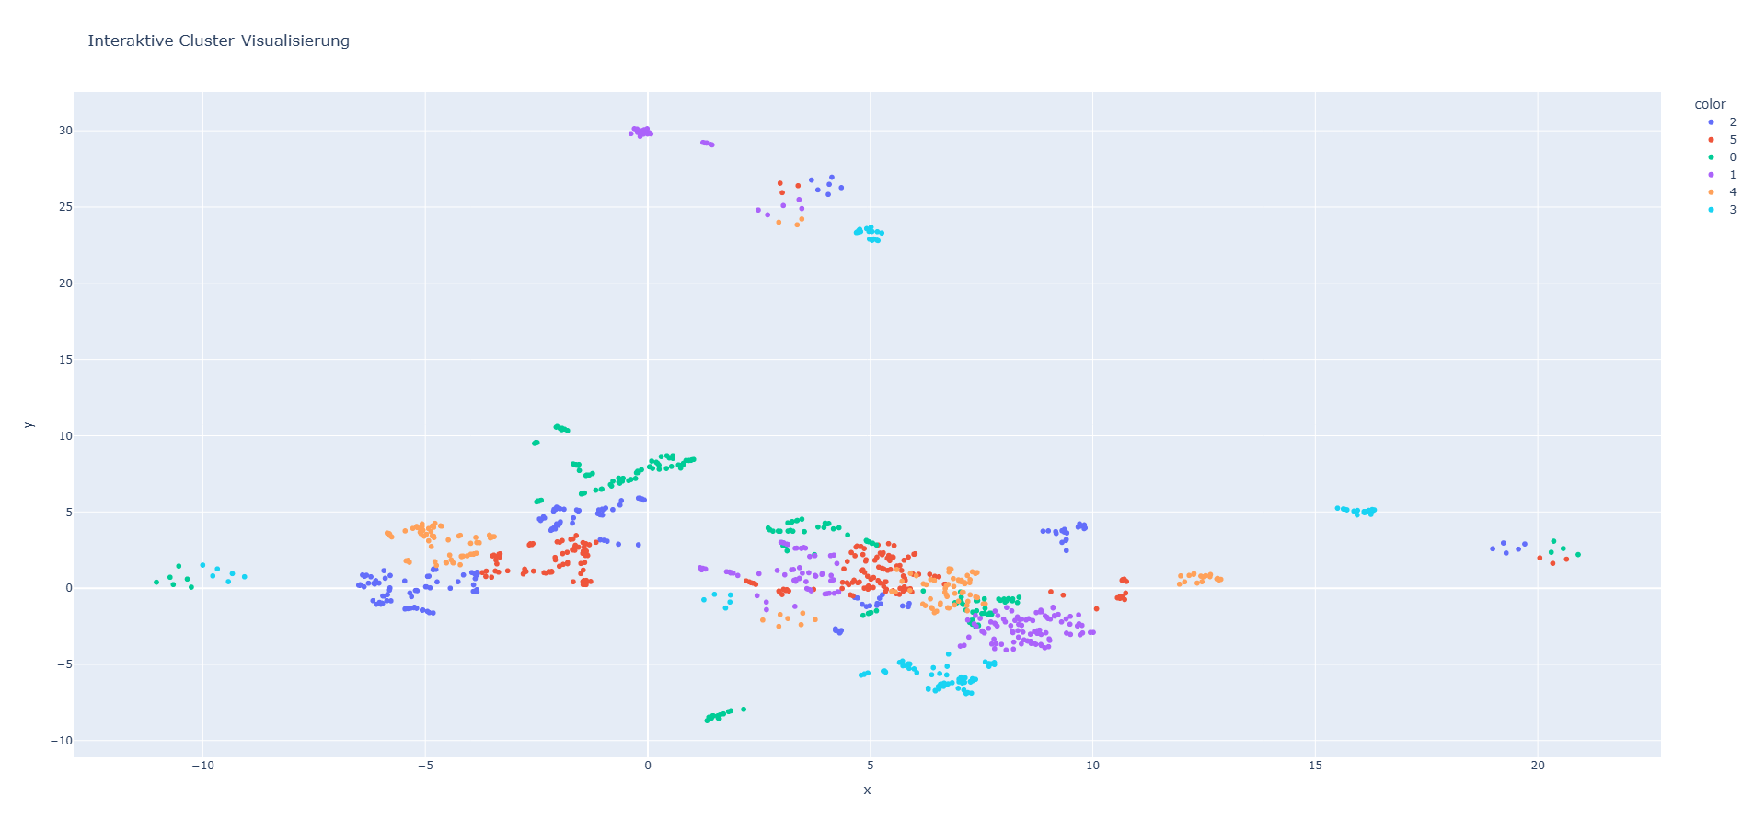
\includegraphics[width=1.0\textwidth]{images/Clusterung - 1000.pdf}
	\caption{Finale Implementierung - Clusterung von rund 1000 Dateien. Pro Farbe wird weiter durch Punktzahlenintervalle unterschieden}
	\label{abb:C-1000}
\end{figure}

\begin{table}[h]
    \centering
    \begin{tabular}{|l|l|l|l|l|l|l|l|l|l|l|l|l|}
    \hline
        Sc.-B. 0-49 & C1 & C2 & C3 & C4 & C5 & C6 & C7 & C8 & C9 & C10 & gl. & ungl. \\ \hline
        Cluster 0: & ~ & ~ & ~ & ~ & ~ & ~ & ~ & ~ & ~ & ~ & ~ & ~ \\ \hline
             0 P & A1 & A1 & A1 & A1 & A1 & A1 & A1 & A1 & A2 & A3 & ~ & ~ \\ \hline
             49 P & A4 & A5 & A4 & A6 & A4 & A5 & A9 & A5 & A7 & A4 & ~ & ~ \\ \hline
        ~ & 0 & 0 & 0 & 0 & 0 & 0 & 0 & 0 & 0 & 0 & 0 & 10 \\ \hline
        Sc.-B. 50-59 & ~ & ~ & ~ & ~ & ~ & ~ & ~ & ~ & ~ & ~ & ~ & ~ \\ \hline
        Cluster 3: & ~ & ~ & ~ & ~ & ~ & ~ & ~ & ~ & ~ & ~ & ~ & ~ \\ \hline
          53 P & A4 & A5 & A4 & A6 & A4 & A5 & A9 & A5 & A7 & A4 & ~ & ~ \\ \hline
          53 P & A1 & A1 & A1 & A1 & A1 & A1 & A1 & A1 & A1 & A8 & ~ & ~ \\ \hline
        ~ & 0 & 0 & 0 & 0 & 0 & 0 & 0 & 0 & 0 & 0 & 0 & 10 \\ \hline
        Sc.-B.  60-74 & ~ & ~ & ~ & ~ & ~ & ~ & ~ & ~ & ~ & ~ & ~ & ~ \\ \hline
        Cluster 1: & ~ & ~ & ~ & ~ & ~ & ~ & ~ & ~ & ~ & ~ & ~ & ~ \\ \hline
          66 P & A1 & A1 & A1 & A6 & A1 & A5 & A9 & A5 & A7 & A4 & ~ & ~ \\ \hline
          70 P & A1 & A1 & A1 & A1 & A1 & A5 & A9 & A5 & A7 & A4 & ~ & ~ \\ \hline
        ~ & 1 & 1 & 1 & 0 & 1 & 1 & 1 & 1 & 1 & 1 & 9 & 1 \\ \hline
        Sc.-B. 75-90 & ~ & ~ & ~ & ~ & ~ & ~ & ~ & ~ & ~ & ~ & ~ & ~ \\ \hline
        Cluster 0: & ~ & ~ & ~ & ~ & ~ & ~ & ~ & ~ & ~ & ~ & ~ & ~ \\ \hline
          75 P & A1 & A1 & A1 & A1 & A1 & A10 & A10 & A10 & A11 & A4 & ~ & ~ \\ \hline
          87 P & A1 & A1 & A1 & A1 & A1 & A1 & A1 & A1 & A7 & A4 & ~ & ~ \\ \hline
        ~ & 1 & 1 & 1 & 1 & 1 & 0 & 0 & 0 & 0 & 1 & 6 & 4 \\ \hline
        Sc.-B. 90-99 & ~ & ~ & ~ & ~ & ~ & ~ & ~ & ~ & ~ & ~ & ~ & ~ \\ \hline
        Cluster 1: & ~ & ~ & ~ & ~ & ~ & ~ & ~ & ~ & ~ & ~ & ~ & ~ \\ \hline
          92 P & A1 & A1 & A1 & A1 & A1 & A1 & A1 & A1 & A1 & A4 & ~ & ~ \\ \hline
          96 P & A1 & A1 & A1 & A1 & A1 & A1 & A12 & A1 & A13 & A1 & ~ & ~ \\ \hline
    \end{tabular}
	\caption{Finale Implementierung - Auswertung der Circle-Dateien}
\label{tab:A-d-CD}
\end{table}

\begin{table}[h]
    \centering
    \begin{tabular}{|l|l|l|l|l|l|l|l|l|}
    \hline
        Sc.-B. 0-49 & P1 & P2 & P3 & P4 & P5 & P6 & gl. & ungl. \\ \hline
        Cluster 0: & ~ & ~ & ~ & ~ & ~ & ~ & ~ & ~ \\ \hline
             0 P & A1 & A4 & A4 & A4 & A4 & A4 & ~ & ~ \\ \hline
             49 P & A15 & A1 & A1 & A1 & A1 & A1 & ~ & ~ \\ \hline
        ~ & 0 & 0 & 0 & 0 & 0 & 0 & 0 & 6 \\ \hline
        Sc.-B. 50-59 & ~ & ~ & ~ & ~ & ~ & ~ & ~ & ~ \\ \hline
        Cluster 3: & ~ & ~ & ~ & ~ & ~ & ~ & ~ & ~ \\ \hline
          53 P & A1 & A1 & A1 & A1 & A1 & A1 & ~ & ~ \\ \hline
          53 P & A4 & A5 & A4 & A5 & A4 & A5 & ~ & ~ \\ \hline
        ~ & 0 & 0 & 0 & 0 & 0 & 0 & 0 & 6 \\ \hline
        Sc.-B.  60-74 & ~ & ~ & ~ & ~ & ~ & ~ & ~ & ~ \\ \hline
        Cluster 1: & ~ & ~ & ~ & ~ & ~ & ~ & ~ & ~ \\ \hline
          66 P & A1 & A1 & A1 & A1 & A1 & A14 & ~ & ~ \\ \hline
          70 P & A1 & A1 & A1 & A1 & A1 & A14 & ~ & ~ \\ \hline
        ~ & 1 & 1 & 1 & 1 & 1 & 1 & 6 & 0 \\ \hline
        Sc.-B. 75-90 & ~ & ~ & ~ & ~ & ~ & ~ & ~ & ~ \\ \hline
        Cluster 0: & ~ & ~ & ~ & ~ & ~ & ~ & ~ & ~ \\ \hline
          75 P & A1 & A1 & A1 & A1 & A1 & A10 & ~ & ~ \\ \hline
          87 P & A1 & A1 & A1 & A1 & A1 & A1 & ~ & ~ \\ \hline
        ~ & 1 & 1 & 1 & 1 & 1 & 0 & 5 & 1 \\ \hline
        Sc.-B. 90-99 & ~ & ~ & ~ & ~ & ~ & ~ & ~ & ~ \\ \hline
        Cluster 1: & ~ & ~ & ~ & ~ & ~ & ~ & ~ & ~ \\ \hline
          92 P & A1 & A1 & A1 & A1 & A1 & A1 & ~ & ~ \\ \hline
          96 P & A1 & A1 & A1 & A1 & A1 & A1 & ~ & ~ \\ \hline
        ~ & 1 & 1 & 1 & 1 & 1 & 1 & 6 & 0 \\ \hline
    \end{tabular}
	\caption{Finale Implementierung - Auswertung der Point-Dateien}
\label{tab:A-d-PD}
\end{table}

\begin{table}[h]
    \centering
    \begin{tabular}{|l|l|}
    \hline
        Aufgaben: & Abkürzungen: \\ \hline
        Circle(Point initLocation, double initRadius) & C1 \\ \hline
        getRadius() & C2 \\ \hline
        setRadius(double newRadius) & C3 \\ \hline
        getLocation() & C4 \\ \hline
        setLocation(Point newLocation) & C5 \\ \hline
        getDiameter() & C6 \\ \hline
        getCircumfence() & C7 \\ \hline
        getArea() & C8 \\ \hline
        containsPoint(Point point) & C9 \\ \hline
        fromPoints(Point center, Point p) & C10 \\ \hline
        ~ & ~ \\ \hline
        Point(double initX, double initY) & P1 \\ \hline
        getX() & P2 \\ \hline
        setX(double newX) & P3 \\ \hline
        getY() & P4 \\ \hline
        setY(double newY) & P5 \\ \hline
        getDistance(Point point) & P6 \\ \hline
        ~ & ~ \\ \hline
        Antworten: & Abkürzungen: \\ \hline
        richtig & A1 \\ \hline
        falsche Einrückung im else-Fall & A2 \\ \hline
        Point hat keine Methode getDiameter() & A3 \\ \hline
        fehlt & A4 \\ \hline
        return -1.0 & A5 \\ \hline
        return new Point() & A6 \\ \hline
        return false & A7 \\ \hline
        center = circle.getLocation(); & A8 \\ \hline
        return Math.PI & A9 \\ \hline
        return 0.0 & A10 \\ \hline
        Quadrat- statt Kreisüberprüfung & A11 \\ \hline
        return Math.PI * getCircumference() & A12 \\ \hline
        if(point.getDistance(location)> getRadius()) & A13 \\ \hline
        Es fehlt eine Klammer bei Math.sqrt() & A14 \\ \hline
        initY = y & A15 \\ \hline
    \end{tabular}
	\caption{Finale Implementierung - Antwortabkürzungen}
\label{tab:Abk}
\end{table}